%!TEX root = ../MasterThesis.tex

\section{Choosing a \gls{RDF} schema}
\label{sec:choose_data_schema}

As a major objective of the \gls{E-commerce} fraud investigation system is to bring the various transactional information from online merchants, \gls{PSP}s and issuers together, combine them and analyze the resulting graph from different view points, the information exchanged between the relevant participants either have to follow a common schema or have to be mapped against each other.

\subsection{Re-using vocabularies available on the Web}
\label{subsec:reuse_vocab_web}

One valid approach to come up with a data schema is to take a look into commonly used \gls{RDF} schemata and vocabularies, and try to figure out whether they can be used for describing the information, that need to be exchanged between participants of the \gls{E-commerce} fraud investigation system. When consulting the Semantic Web community for commonly agreed upon and highly used \gls{RDF} schema specifications, one will come up with this list (see Table~\ref{tab:used_vocab_rdf}):\@

\begin{table}[H]
\centering
\begin{tabular}{p{3cm}llp{4.5cm}}
\hline
\textbf{Name} & \textbf{Prefix} & \textbf{Describes} & \textbf{Namespace URI} \\
\hline
Dublin Core & dc: & Meta data & \url{http://purl.org/dc/terms/} \\
\hline
FOAF & foaf: & People & \url{http://xmlns.com/foaf/0.1/} \\
\hline
Geo & pos: & Positions & \url{http://www.w3.org/2003/01/geo/wgs84\_pos\#} \\
\hline
Geo Names & gn: & Locations & \url{http://www.geonames.org/ontology\#} \\
\hline
Good Relations & gr: & Products & \url{http://purl.org/goodrelations/v1\#} \\
\hline
RDF & rdf: & Core framework & \url{http://www.w3.org/1999/02/22-rdf-syntax-ns\#} \\
\hline
RDFS & rdfs: & RDF vocabularies & \url{http://www.w3.org/2000/01/rdf-schema\#} \\
\hline
Schema.org & schema: & Schema.org vocabularies & \url{http://schema.org/} \\
\hline
SKOS & skos: & Controlled vocabularies & \url{http://www.w3.org/2004/02/skos/core\#} \\
\hline
vCard & vcard: & Business Cards & \url{http://www.w3.org/2006/vcard/ns\#} \\
\hline
Web Ontology Language & owl: & Ontologies & \url{http://www.w3.org/2002/07/owl\#} \\
\hline
XML Schema Datatypes & xsd: & Data types & \url{http://www.w3.org/2001/XMLSchema\#} \\
\hline
\end{tabular}
\caption[Commonly used \gls{RDF} vocabularies on the Web]{Commonly used \gls{RDF} vocabularies on the Web \citep[pg. 41]{wood2014linked}}
\label{tab:used_vocab_rdf}
\end{table}

Based on these schema specifications describing a fictive consumer named ``Max Mustermann'' incl.\ his home address can be done by combining data utilizing the \gls{FOAF} and \gls{vCard} namespaces in a \gls{RDF} data set, such as described in Listing~\ref{lst:sample_customer_mustermann} and visualized as graph in Figure~\ref{fig:images_sample_customer}. \@

\begin{listing}[H]
  \inputminted[linenos,
               numbersep=5pt,
               breaklines=true,
               frame=lines]{TURTLE}
               {./samples/sample_customer_mustermann.ttl}
  \caption{Personal related information about a fictive consumer in \gls{RDF}}
\label{lst:sample_customer_mustermann}
\end{listing}

\begin{figure}[H]
	\centering
		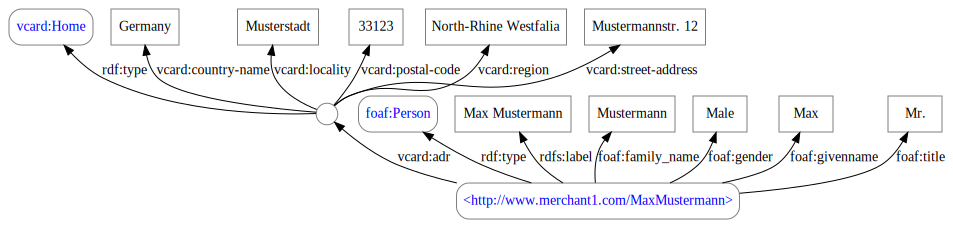
\includegraphics[width=\columnwidth]{images/sample_customer_mustermann.pdf}
	\caption{Graph representation of consumer information from Listing~\ref{lst:sample_customer_mustermann}}
\label{fig:images_sample_customer}
\end{figure}

Looking back to the initial data model from Section~\ref{sec:data_model_transactions} one can map the information, that are currently available in the \gls{E-commerce} scenario, to the existing \gls{RDF} vocabularies such as follows (see Table~\ref{tab:map_tx_rdf_vocab}):\@

\begin{table}[H]
\centering
\begin{tabular}{p{5cm}l}
\hline
\textbf{Information} & \textbf{RDF vocabulary} \\
\hline
Consumer & FOAF \\
\hline
Credit Card Owner & FOAF \\
\hline
Billing Address & vCard \\
\hline
Shipping Address & vCard \\
\hline
Location Information & Geo Names \\
\hline
Merchant & GoodRelations \\
\hline
Items & GoodRelations \\
\hline
Item Categories & GoodRelations \\
\hline
Brands & GoodRelations \\
\hline
Payment Types & GoodRelations \\
\hline
\end{tabular}
\caption{Possible usage of \gls{RDF} vocabularies for \gls{E-commerce} transaction information}
\label{tab:map_tx_rdf_vocab}
\end{table}

As this table shows there are some parts of the \gls{E-commerce} data model that can be expressed with existing \gls{RDF} vocabularies extensively --- such as personal related information via \gls{FOAF} and \gls{vCard}, whereas other parts can not be stated in-depth (e.g. credit card information), or are not specified at all (e.g.\ tracking of the delivery). Additionally some of the vocabularies are no longer actively maintained, such as GoodRelations. Due to these circumstances one usually have to build an own ontology that fills in the missing pieces and refers to the existing concepts whenever appropriate.

% subsection reuse_vocab_web (end)

\subsection{Creating a vocabulary for \gls{E-commerce} transactions}
\label{subsec:build_ontology_frauds}

Another possible approach is to define a completely new schema for the proposed system and share that with every possible stakeholder. This schema will define all the entities and relations known to the collaborative system and would be expressed in \gls{RDFS} format. \\

Trying to model the information of a credit card as displayed in Figure~\ref{fig:images_data_model} will result in the \gls{RDFS} specification shown in Listing~\ref{lst:credit_card_vocab}. This definition of a credit card resource explicitly reuses specifications from the \gls{FOAF} and GoodRelations ontologies by specifying that: \@

\begin{itemize}
 \item the owner of a credit card has to be of type ``Person'' from the \gls{FOAF} ontology
 \item the type of a credit card has to be an instance of the type ``PaymentMethodCreditCard'' from the GoodRelations ontology
\end{itemize}

\begin{listing}[H]
 \inputminted[linenos,
              numbersep=5pt,
              breaklines=true,
              frame=lines]{TURTLE}
              {./samples/vocab_credit_card.ttl}
 \caption{A specification for a credit card in \gls{RDFS}}
\label{lst:credit_card_vocab}
\end{listing}

As most of the parts of the \gls{E-commerce} data model shown in Figure~\ref{fig:images_data_model} can not be expressed directly with the existing \gls{RDF} vocabularies, filling in the gaps would mean to come up with a large set of custom entities and relationships. A major drawback of this approach is, that new partners of the system will first have to implement the conversion of their internal data structures to an \gls{RDF} data set, that is compatible with the specific schema definition, before being able to participate in it. This will limit the general usage of the collaborative system.

% subsection build ontology (end)

\subsection{Schema.org initiative}
\label{subsec:schema_org}

When looking back at the list of existing ontologies and vocabularies, that are actively used on the Web today, one will also find the Schema.org vocabulary definition \citep{Schema.org}. This vocabulary was initially designed by the leading search engines (e.g.\ Google, Microsoft and Yahoo!) to allow authors of Web sites to markup their \gls{HTML} documents in a way, that they are better understood by these search engines. The Schema.org vocabulary is actively maintained by its community, includes new concepts with each release and also offers an extension mechanism to implement additional vocabularies with terms, that are not part of the core specification \citep{SchemaExtensions}. In one of the past releases of the Schema.org core specification the maintainers also included all of the existing concepts of the GoodRelation ontology into the Schema.org vocabulary \citep{SchemaGoodRelation}. \\

As the merchants will likely provide semantic meta data for their products to improve their listings on search engine results (also known as \gls{SEO}) using the vocabulary of Schema.org already, one can re-use parts of these information for the \gls{E-commerce} fraud investigation scenario. Additionally, the wide-ranging scope of aspects declared in the Schema.org vocabulary, make it a good fit for the collaborative system of the \gls{E-commerce} fraud investigation scenario as one can assume, that each participant is aware of this meta data initiative, and the relevant communication partners will have a common understanding of the terms declared in that system. When trying to map the initial data model from Section~\ref{sec:data_model_transactions} to the Schema.org core specification, one will basically come up with a schema as displayed in Figure~\ref{fig:images_schema_org}. \@

\begin{figure}[!ht]
	\centering
		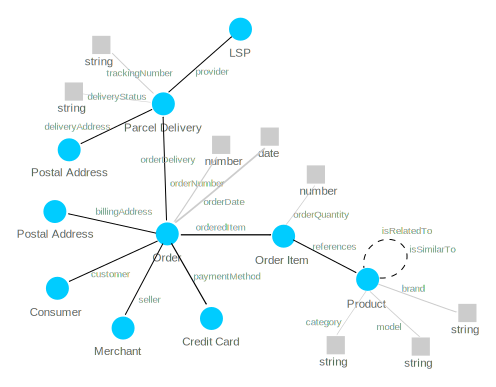
\includegraphics[width=0.8\columnwidth]{images/schema_org_mapping.pdf}
	\caption{Schema.org based mapping of an \gls{E-commerce} transaction}
\label{fig:images_schema_org}
\end{figure}

% subsec schema_org (end)

% sec data_schema (end)
